\section{Supplementary tables}

\begin{table}[h]
\caption[Optimal classifier parameters]{Support vector machine parameter summary}
\begin{center}
	\begin{tabular*}{\textwidth}{l @{\extracolsep{\fill}} ll}
	\hline
	Parameter	                     & Optimal value/algorithm       \\ 
	\hline
	Feature selection algorithm     & ReliefF     \\
	k-ReliefF         & 80        \\
	Number of features                     & 20             \\
	Cross-validation       & 3-fold cross-validation          \\
	Class balance      & Inverse of class frequencies           \\
	Observation weights       & Drug side effect frequency per drug           \\
	SVM kernel       & Gaussian           \\
	\hline
	\end{tabular*}
\end{center}
\label{tbl:tbls1ch2}%descriptive label to refer to figure in text
\end{table}

\newpage

\begin{table}[h]
\caption[Automatically optimized SVM hyperparameters.]{Automatically optimized SVM hyperparameters.}
\begin{center}
	\begin{tabular*}{\textwidth}{l @{\extracolsep{\fill}} ll}
	\hline
	Hyperparameter	                     & Value/Range       \\ 
	\hline
	Standardize data     & True,false     \\
	Kernel         & Linear, Gaussian, polynomial        \\
	Polynomial order                     & [2,5]             \\
	Box constraints       & [1e-6,1e+4]         \\
	Kernel scale      & True,false          \\
	\hline
	\end{tabular*}
\end{center}
\label{tbl:tbls2ch2}%descriptive label to refer to figure in text
\end{table}

\newpage
\newpage

\begin{table}[h]
\caption[Area under the ROC curve of the predicted side effect.]{Area under the ROC curve of the predicted side effect using a multi-label support vector machine classifier with combined gene expression and sampled metabolic flux as features.}
\begin{center}
	\begin{tabular*}{\textwidth}{l @{\extracolsep{\fill}} ll}
	\hline
	Side effect	                     & AUROC       \\ 
	\hline
Gastrointestinal pain                 & 0.52\\
Gastrointestinal disorder             & 0.53\\
Functional gastrointestinal disorder  & 0.63\\                 
Gastrointestinal haemorrhage          & 0.64\\    
Intestinal obstruction                & 0.67\\     
Intestinal perforation                & 0.69\\  
Gastrointestinal tract irritation     & 0.72\\ 
Gastrointestinal perforation          & 0.74\\ 
Gastrointestinal obstruction          & 0.75\\   
Gastrointestinal fistula              & 0.79\\
Intestinal ulcer                      & 0.8\\   
Gastrointestinal hypomotility         & 0.8\\        
Gastrointestinal sounds abnormal      & 0.9\\ 
Gastrointestinal ulcer haemorrhage    & 0.9\\     
Gastrointestinal infection            & 0.91\\
Gastrointestinal necrosis             & 0.92\\ %%  
Gastrointestinal toxicity             & 0.92\\ 
Upper gastrointestinal haemorrhage    & 0.93\\ 
Lower gastrointestinal haemorrhage    & 0.95\\
Gastrointestinal carcinoma            & 0.96\\
Gastrointestinal ulcer perforation    & 0.96\\
Gastrointestinal motility disorder    & 0.97\\ 
Intestinal infarction                 & 0.97\\
Gastrointestinal ulcer                & 0.97\\
Gastrointestinal stromal tumour       & 0.97\\
Pneumatosis intestinalis              & 0.97\\           
Intestinal ischaemia                  & 0.98\\      
Large intestine polyp                 & 0.98\\ 
Gastrointestinal malformation         & 0.98\\ %%   
Gastrointestinal candidiasis          & 0.99\\   
Benign gastrointestinal neoplasm      & 0.99\\  
Gastrointestinal inflammation         & 0.99\\  
Diverticulum intestinal               & 0.99\\   
Large intestine perforation           & 0.99\\  
Small intestinal obstruction          & 0.99\\  
Intestinal haemorrhage                & 0.99\\  
	\hline
	\end{tabular*}
\end{center}
\label{tbl:tbls3ch2}%descriptive label to refer to figure in text
\end{table}

\clearpage
\section{Supplementary figures}
\begin{figure}[!htp]
\centering
	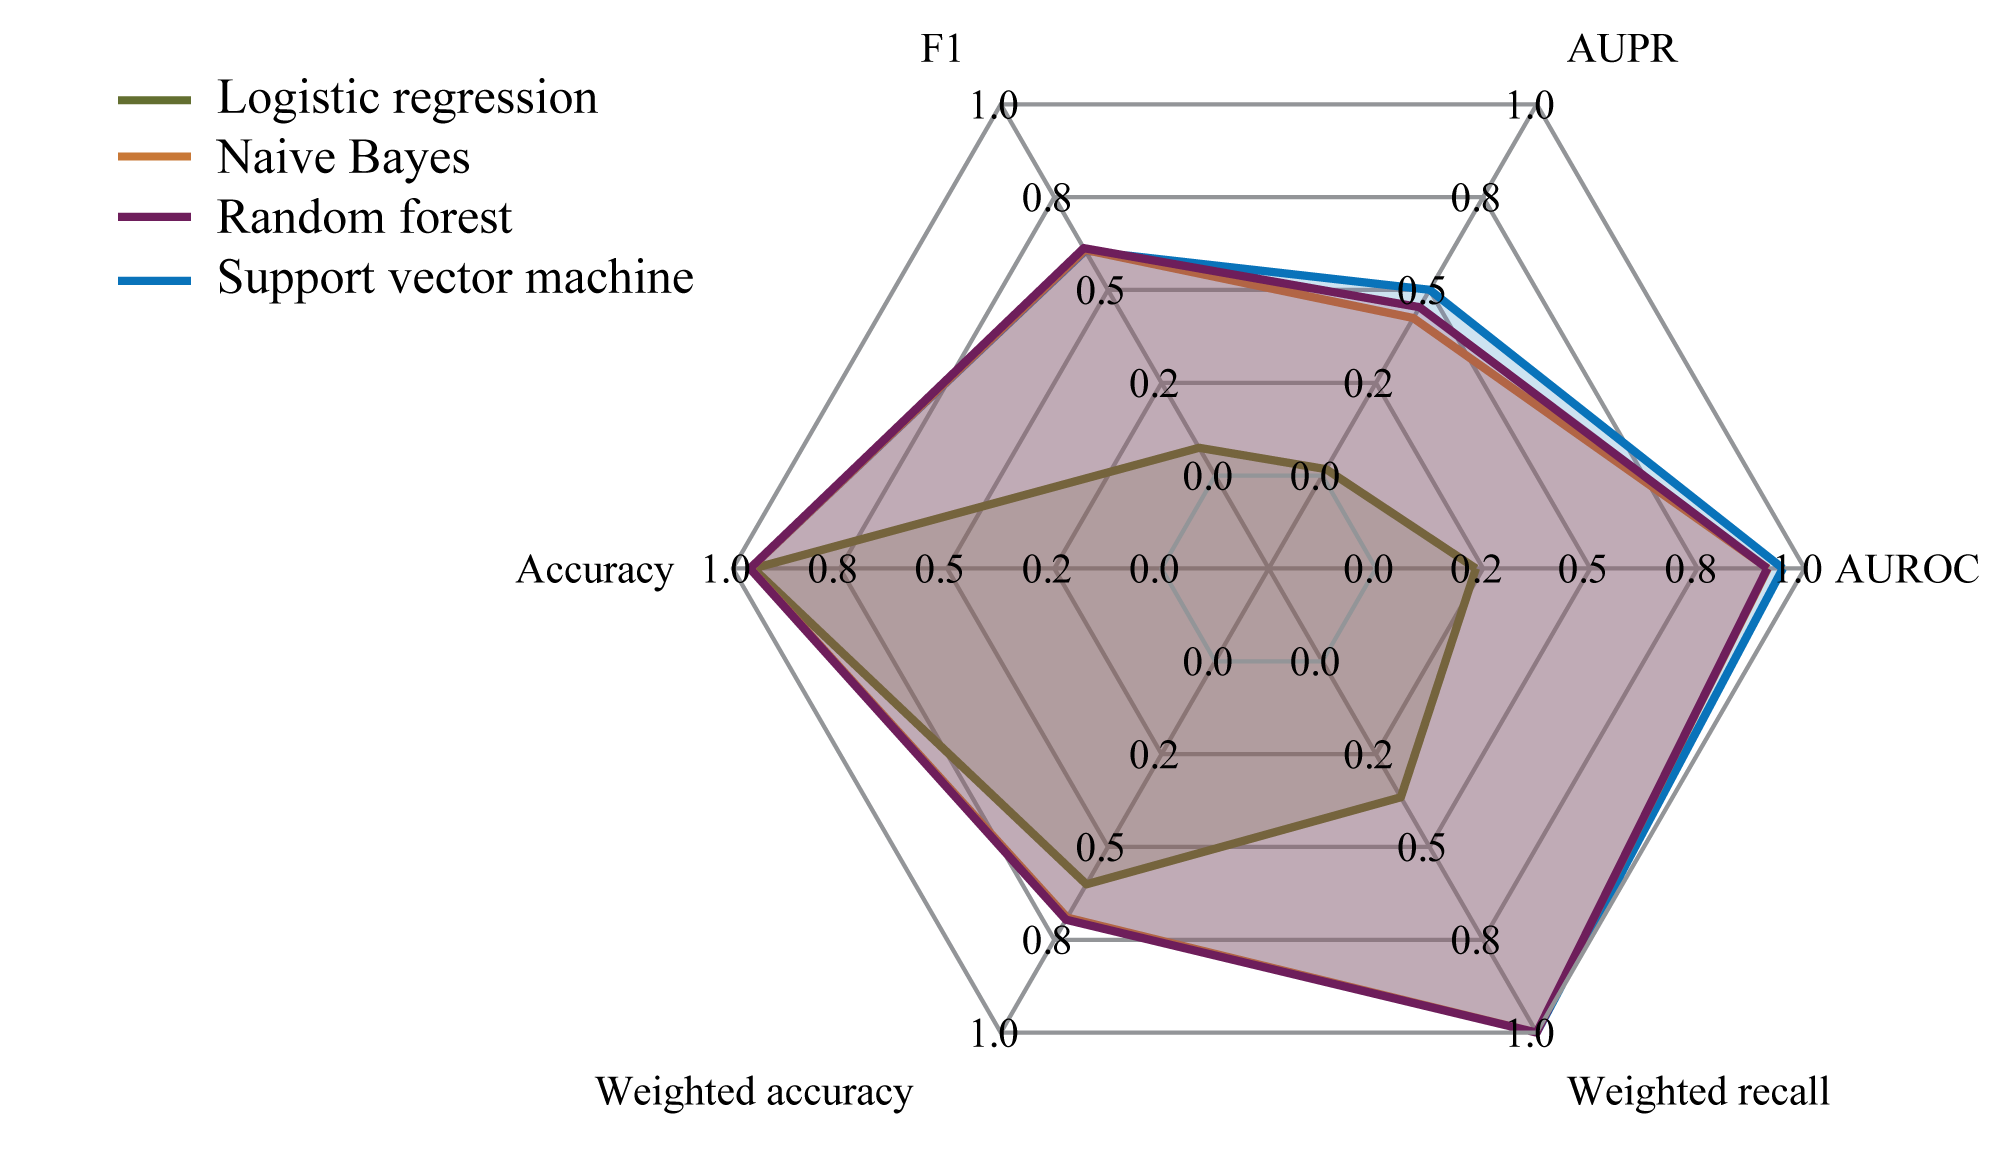
\includegraphics[width=\textwidth,height=\textheight,keepaspectratio]{sideEffects/Algorithms.png}%Figure from images\Figure1.png
	\caption[Comparison of multi-label classifiers.]{Comparison of multi-label classifiers. Four classifiers namely, logisitic regression, naive Bayes, random forest, and support vector machine were compared in their predictive capabilities measured by the F1-score, accuracy,class weighted accuracy, class weighted recall, area under the ROC curve (AUROC), area under the precision-recall curve (PR).}
	\label{fig:s1algo}
\end{figure}

\clearpage
\begin{figure}[!htp]
\centering
	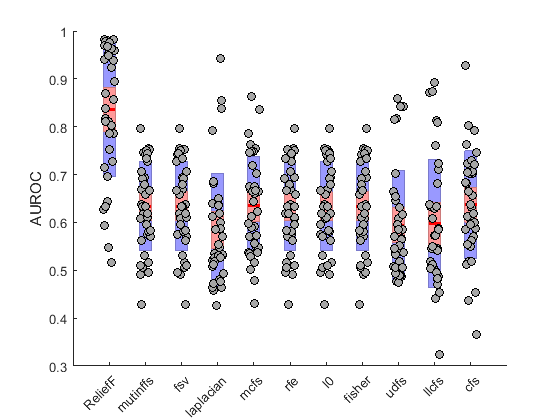
\includegraphics[width=\textwidth,height=\textheight,keepaspectratio]{sideEffects/figS1.png}%Figure from images\Figure1.png
	\caption[Feature selection algorithm comparison.]{Comparison of 11 feature selection algorithm with respect to the area under the ROC curve of individual intestinal side effects with the 95\% confidence interval for the mean in red and one standard deviation in blue.}
	\label{fig:s1seff}
\end{figure}

\clearpage
\begin{figure}[!htp]
\centering
	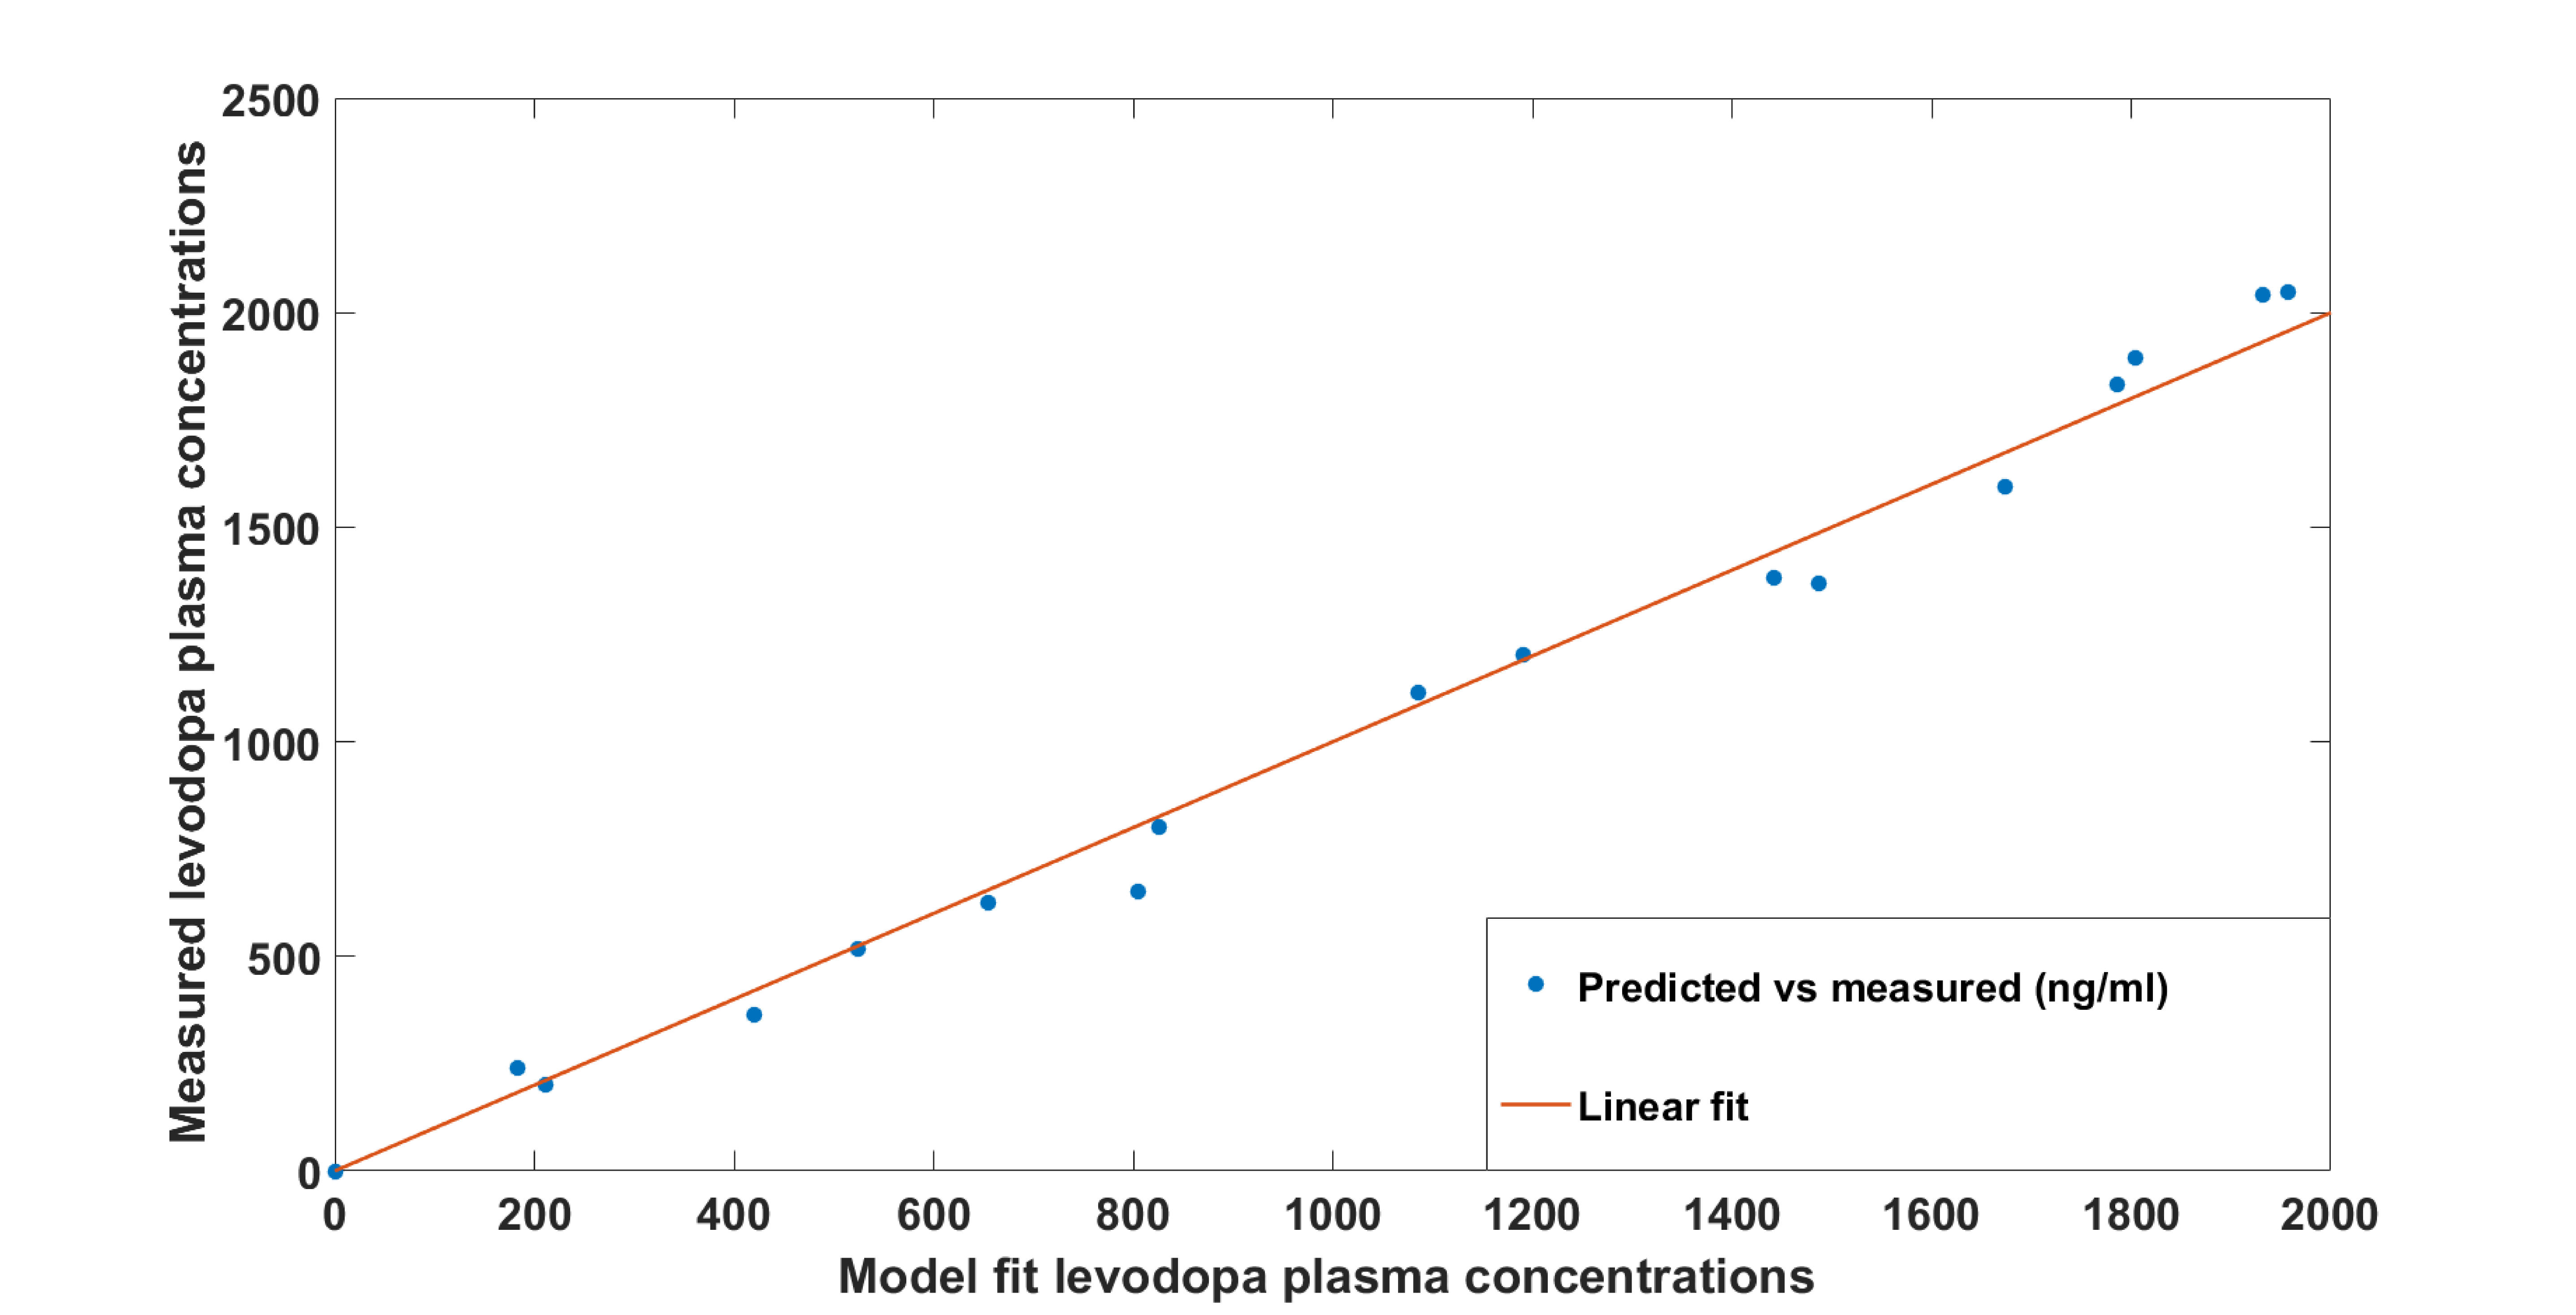
\includegraphics[width=\textwidth,height=\textheight,keepaspectratio]{sideEffects/figS2.png}%Figure from images\Figure1.png
	\caption[ReliefF's k value comparison.]{Comparison of k values for the feature selection algorithm ReliefF through the area under the ROC curve of classifiers of individual side effects with the 95\% confidence interval for the mean in red and one standard deviation in blue. The highest mean (0.83) was achieved for k=80.}
	\label{fig:s2seff}
\end{figure}

\clearpage
\begin{figure}[!htp]
\centering
	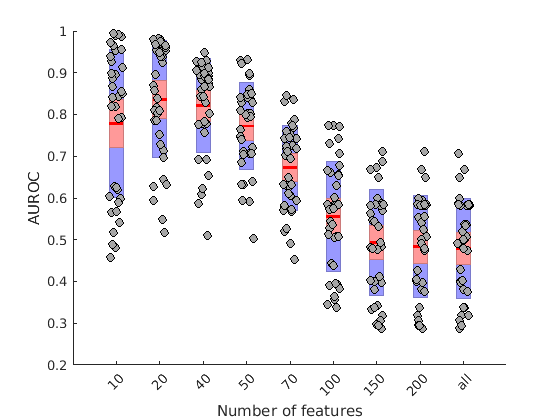
\includegraphics[width=\textwidth,height=\textheight,keepaspectratio]{sideEffects/figS3.png}%Figure from images\Figure1.png
	\caption[Comparison of the number of selected features.]{Comparison of the effect of the number of the most predictive features on the classification performance as assessed by the area under the ROC curve.}
	\label{fig:s3seff}
\end{figure}

\clearpage
\begin{figure}[!htp]
\centering
	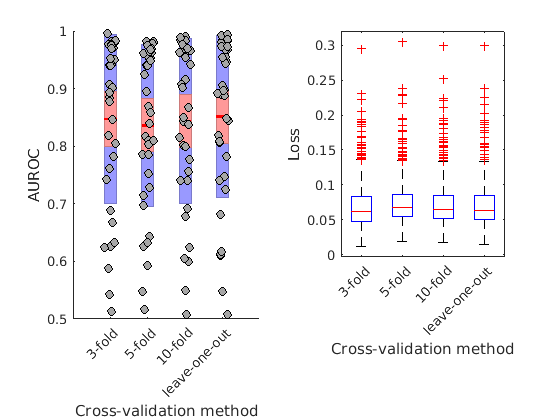
\includegraphics[width=\textwidth,height=\textheight,keepaspectratio]{sideEffects/figS4.png}%Figure from images\Figure1.png
	\caption[Assessment of the cross-validation loss.]{Comparison of cross-validation method on the loss computed as the number of misclassified side effects per drugs over the total number of side effects, and the predictability of the individual side effects as reflected by area under the ROC curve (AUROC). Outliers in the loss are rare side effects that have a small number of data points. The 3-fold cross-validation ensured a lower loss and the highest area under the ROC curve on out-of-sample drugs. Left: distribution of AUROC of individual side effects with the 95\% confidence interval for the mean in red and one standard deviation in blue. Right: boxplot of the loss computed for each cross-validation method.}
	\label{fig:s4seff}
\end{figure}

\clearpage
\begin{figure}[!htp]
\centering
	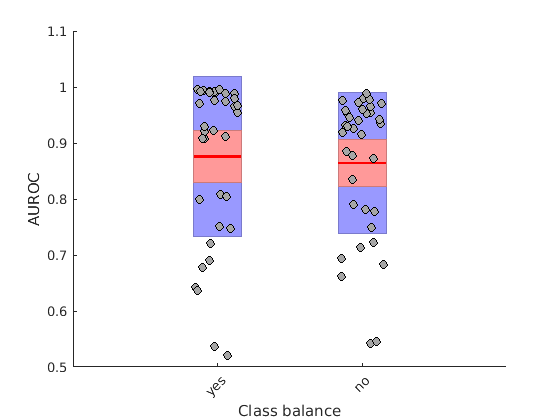
\includegraphics[width=\textwidth,height=\textheight,keepaspectratio]{sideEffects/figS5.png}%Figure from images\Figure1.png
	\caption[Effect of class balance.]{Comparison of the effect of class balance set as the misclassification cost, on the outcome of the classification as determined by the area under the ROC curve. The misclassification cost, set to the inverse of class frequencies, allowed to obtain a mean of 0.875 of the AUROC of the individual intestinal side effects as opposed to 0.86 without class balance.}
	\label{fig:s5seff}
\end{figure}

\clearpage
\begin{figure}[!htp]
\centering
	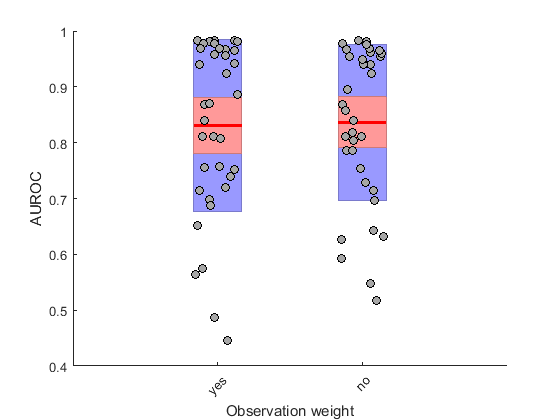
\includegraphics[width=\textwidth,height=\textheight,keepaspectratio]{sideEffects/figS6.png}%Figure from images\Figure1.png
	\caption[Effect of observation weight.]{Comparison of the effect of adding observation weights to the classifier as compared the area under the ROC curve. The weights of drugs per class were set to their frequencies reported in SIDER. Weighing observations has a mean area under the curve of 0.830 while unweighted observation has a mean of 0.836.}
	\label{fig:s6seff}
\end{figure}

\clearpage
\begin{figure}[!htp]
\centering
	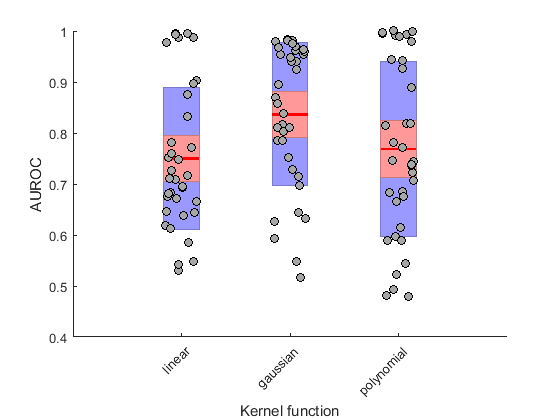
\includegraphics[width=\textwidth,height=\textheight,keepaspectratio]{sideEffects/figS7.png}%Figure from images\Figure1.png
	\caption[Comparison of SVM kernel functions.]{Comparison of SVM kernel functions as a function of area the under the ROC curve of individual side effects. Over all, the Gaussian kernel had the highest predictive capabilities.}
	\label{fig:s7seff}
\end{figure}

\clearpage
\begin{figure}[!htp]
\centering
	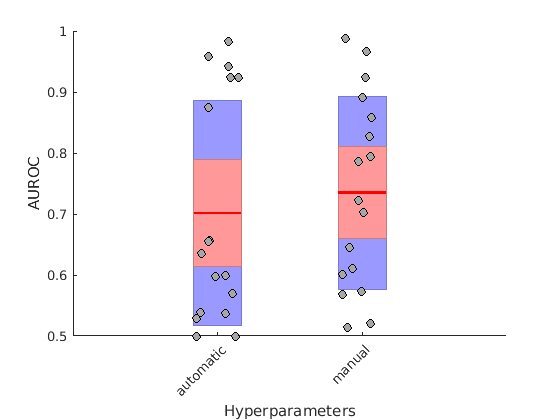
\includegraphics[width=\textwidth,height=\textheight,keepaspectratio]{sideEffects/figS8.png}%Figure from images\Figure1.png
	\caption[Automatic tuning of kernel parameters.]{Effect of automatic and manual hyperparameter optimisation with respect to 20\% holdout accuracy as an objective function. The manually obtained parameters allowed for a higher predictive capability of the classifier as measured by the individual side effect area under the ROC curve.}
	\label{fig:s8seff}
\end{figure}

\clearpage
\begin{figure}[!htp]
\centering
	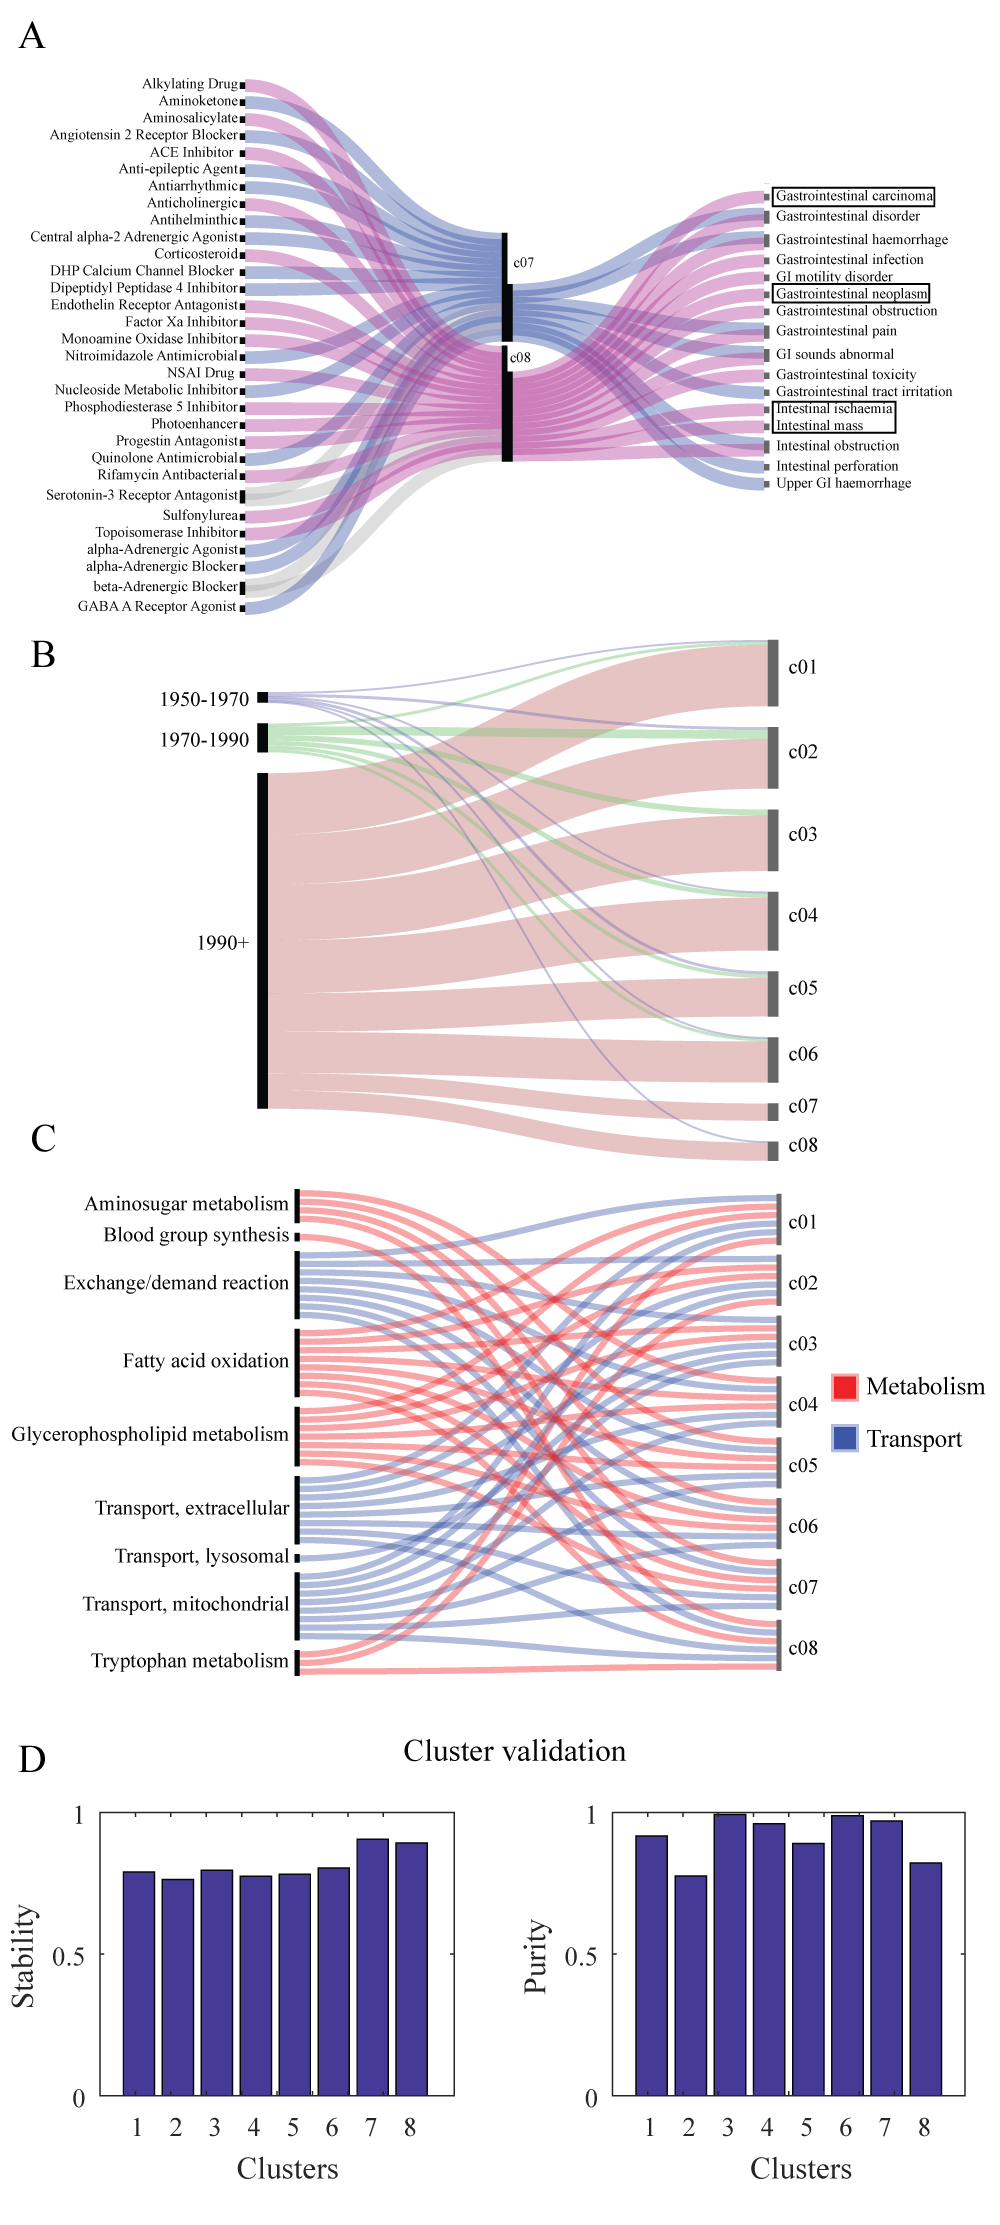
\includegraphics[width=\textwidth,height=\textheight,keepaspectratio]{sideEffects/figS9.png}%Figure from images\Figure1.png
	\caption[Drug cluster validation and characteristics]{(Continued on the following page)}
	\label{fig:s9seff}
\end{figure}
\begin{figure}[t]
  \contcaption{Drug cluster validation and characteristics. A- Graph linking drug clusters, intestinal side effects and FDA NDCD’s established pharmacological class (EPC). B- Bipartite graph of drug clusters and the corresponding FDA NDCD’s reported marketing date. C-Bipartite graph of drug clusters and enriched metabolic and transport subsystems. The flow chart was done using Rawgraphs \cite{Mauri:2017:RVP:3125571.3125585}. E-Cluster stability and purity provided a means for cluster validation.}% Continued caption
\end{figure}
